\documentclass[11pt,twocolumn,twoside]{opticajnl}
%% Please use 11pt if submitting to AOP
% \documentclass[11pt,twocolumn,twoside]{opticajnl}

\journal{pr} % Choose journal (ao,jocn,josaa,josab,ol,optica,pr)

%See template introduciton for guidance on setting shortarticle option
\setboolean{shortarticle}{True}
% true = letter/tutorial
% false = research/review article
% (depending on journal)
\usepackage{lineno}
\usepackage[utf8]{inputenc}
\spanishdecimal{.}
\usepackage{amsmath}
\usepackage{caption}
\usepackage{subcaption}
\usepackage[spanish]{babel}
\usepackage{hyperref}
\usepackage{listings}
\usepackage{multicol}
%\linenumbers

% Configura el formato del título del listado
\renewcommand\lstlistingname{Código}
\renewcommand\lstlistlistingname{Códigos}
\title{
\vspace{0.1cm} 

Trabajo práctico 3: Aprendizaje supervisado en redes multicapa}

\author[1]{\huge{Ignacio Lembo Ferrari}}
\affil[1]{\large{ignaciolembo@ib.edu.ar} 

\vspace{0.1cm}

{\datesfont 14 de octubre de 2023.}

\vspace{0.1cm}
}

%\begin{abstract}
%\textbf{hola}
%\end{abstract}

\begin{document}

\maketitle

El algoritmo de aprendizaje supervisado llamado retropropagación (\textit{backpropagation}) es clave en el desarrollo de las redes neuronales. Dicho algoritmo, que tiene como base el algoritmo \textit{gradient-descent}, da una prescripción para actualizar los pesos $w_{ij}$ en cualquier red \textit{feed-forward} con el objetivo de aprender un conjunto de pares entrada-salida. 

Se puede mostrar que, utilizando retropropagación, se pueden entrenar redes neuronales multicapa para que \textit{aprendan} alguna función. En particular, una red neuronal con una capa oculta se puede utilizar para representar cualquier función Booleana, como por ejemplo el XOR. En este trabajo, en las secciones \ref{sec:ej1} y \ref{sec:ej2}, se implementó en Python una red neuronal con una capa oculta y se utilizó el algoritmo de \textit{backpropagation} desarrollado en el libro de Hertz, Krough y Palmer para resolver la lógica del XOR y el problema de paridad. En la sección \ref{sec:ej3} se utilizó la librería \texttt{Keras} del paquete de Python llamado \texttt{tensorflow} para entrenar una red que aprenda el mapeo logístico.

Para las secciones \ref{sec:ej1} y \ref{sec:ej2} se define el error cuadrático medio (\textit{root mean square error} o MSE) como
\begin{equation}
    E[\boldsymbol{w}] = \frac{1}{2} \sum_{\mu,i} \left[ \zeta_i^{\mu} - O_i^{\mu} \right]^2,
\end{equation}
donde $\mu$ es el índice de los pares entrada-salida de entrenamiento $(\xi_i^\mu, \zeta_i^\mu)$, $i$ es el índice de las neuronas de la capa de salida y $O_i^{\mu}$ es la salida de la red para la entrada $\xi_i^\mu$. Además, la precisión de la red se define como la fracción de pares entrada-salida que la red clasifica correctamente. Se considera correcto si la salida de la red tiene un error realitivo menor o igual al $10\%$ respecto a la salida deseada. Además, en ambas secciones se utilizó como función de activación de las neuronas de la capa oculta y de salida la función $\tanh(x)$. 


\section{Aprendizaje lógica XOR \label{sec:ej1}}

\vspace{0.3cm}

La regla XOR tiene dos entradas ($+1$ o $-1$) y la salida es $-1$ si ambos son diferentes y $1$ si son iguales. Utilizando el algoritmo de retropropagación, se resolvió este problema para las dos arquitecturas mostradas en la Fig. \ref{fig:esq_1}. Las arquitecturas de la Figs. \ref{fig:esq_1}A y \ref{fig:esq_1}B se dominarán 2-2-1 y 2-1-1 respectivamente, en base a la cantidad de neuronas de cada capa. 

\begin{figure}[ht]
    \centering
         \begin{subfigure}[b]{0.75\linewidth}
            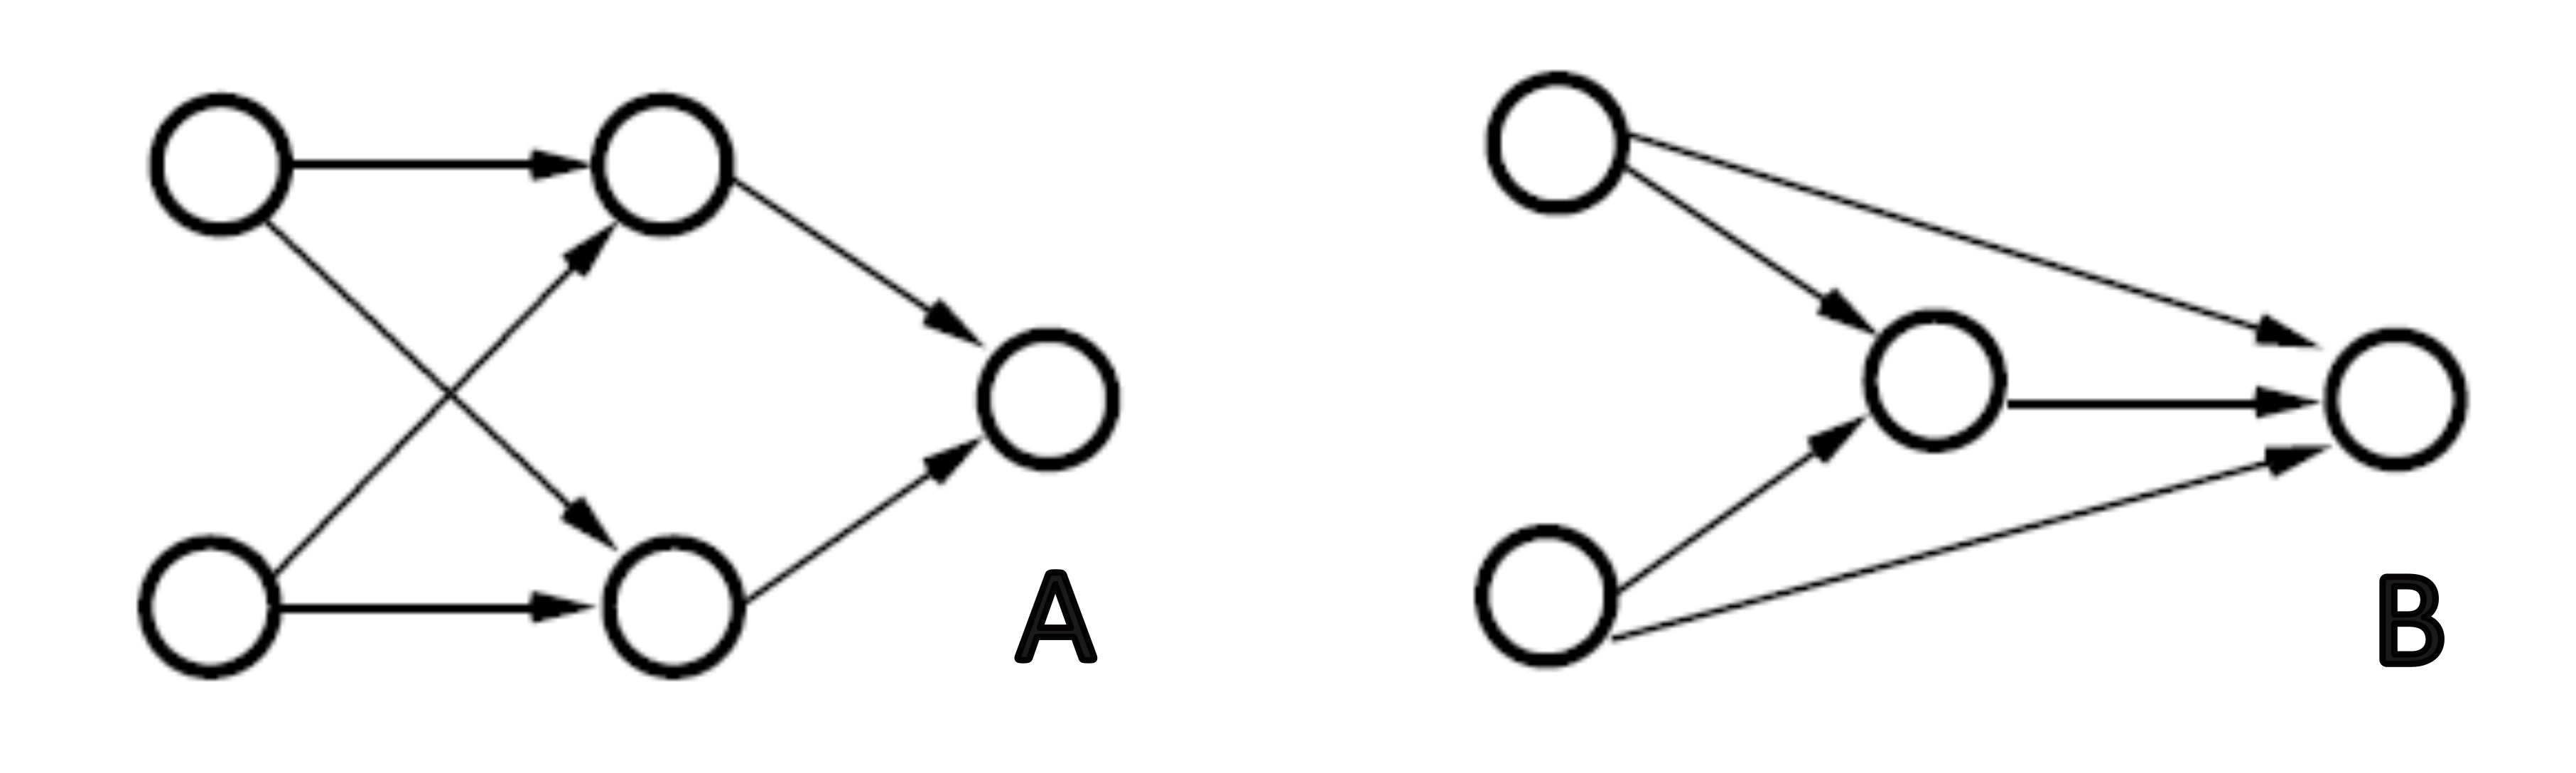
\includegraphics[width=\textwidth]{Figuras/esquema1.png}
         \end{subfigure}
    \caption{Arquitecturas implementadas para resolver la lógica del XOR. (A) Arquitectura $2-2-1$. (B) Arquitectura $2-1-1$.} 
    \label{fig:esq_1}
\end{figure}

Se utilizaron las cuatro posibles entradas del XOR para el entrenamiento de la red, se utilizó una tasa de aprendizaje de $\eta = 0.05$ y se entrenó la red durante $10000$ épocas. Se repitió el entrenamiento 10 veces para valores iniciales distintos de los pesos. Además se agregó un umbral o \textit{bias} a cada neurona de la capa oculta y de salida. Este umbral se representó como una neurona de salida $+1$ y conectada con pesos a todas las neuronas con \textit{bias}. En la Fig. \ref{fig:1} se muestran el MSE y la precisión obtenidos en función de la épocas para ambas arquitecturas. 

\begin{figure}[h]
    \centering
         \begin{subfigure}[b]{0.49\linewidth}
            \centering
            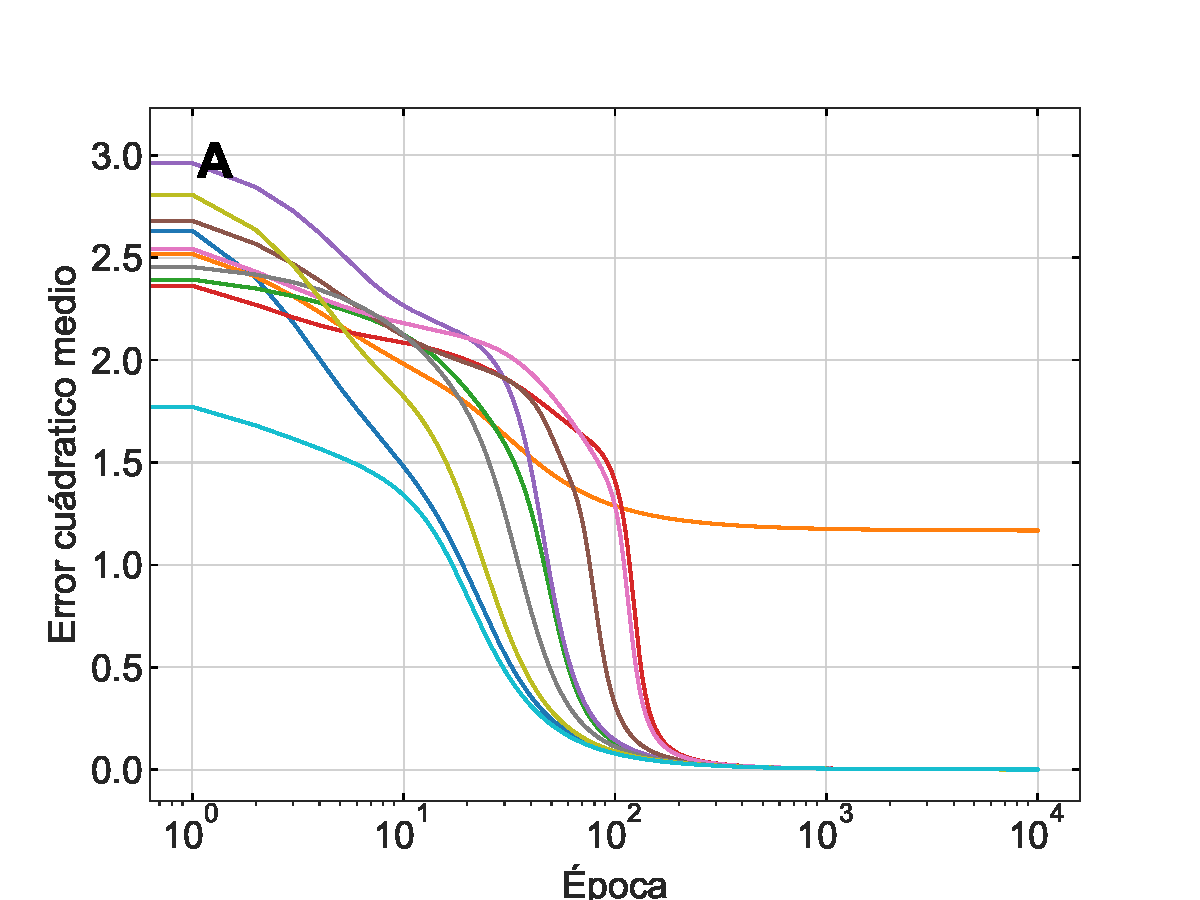
\includegraphics[width=1.1\textwidth]{Figuras/mse_ej1a.pdf}
         \end{subfigure}
         \begin{subfigure}[b]{0.49\linewidth}
            \centering
            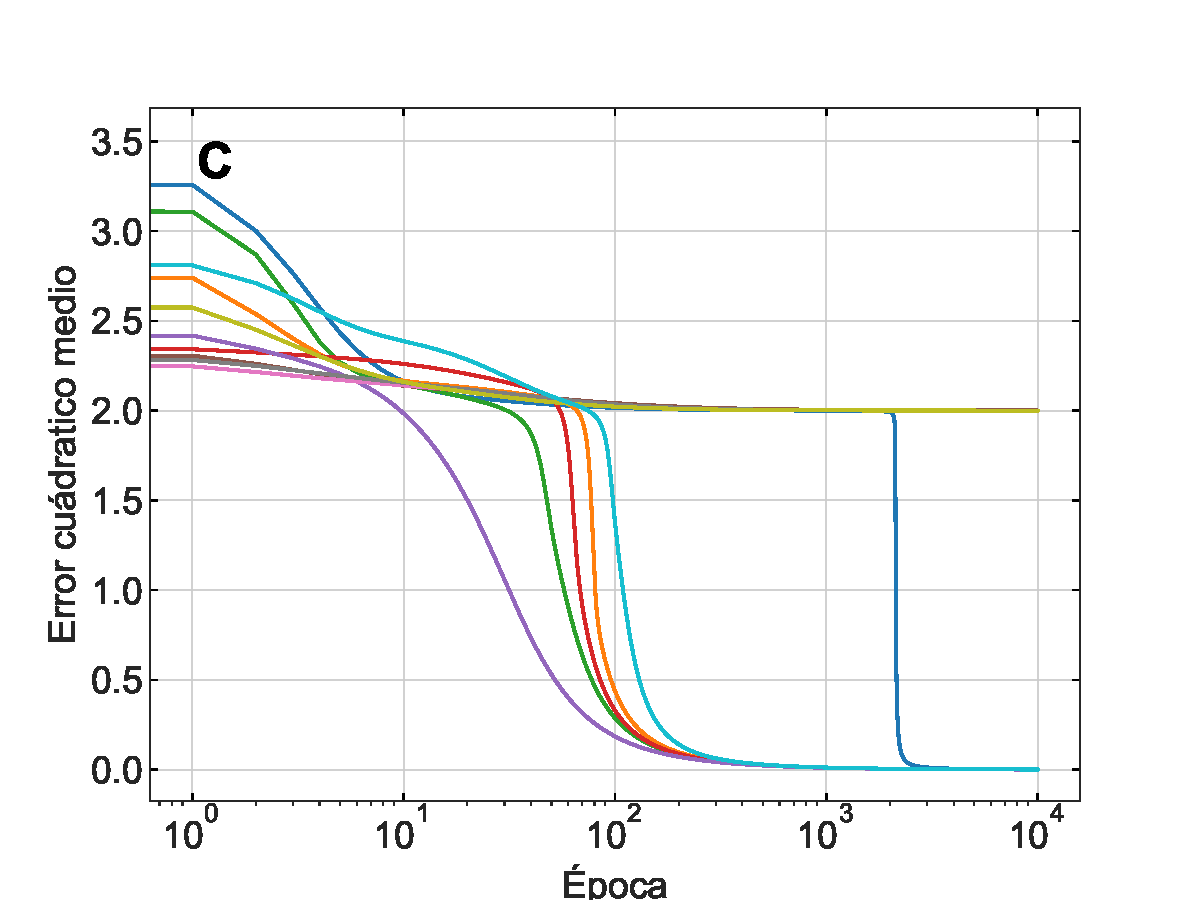
\includegraphics[width=1.1\textwidth]{Figuras/mse_ej1b.pdf}
         \end{subfigure}
         \begin{subfigure}[b]{0.49\linewidth}
            \centering
            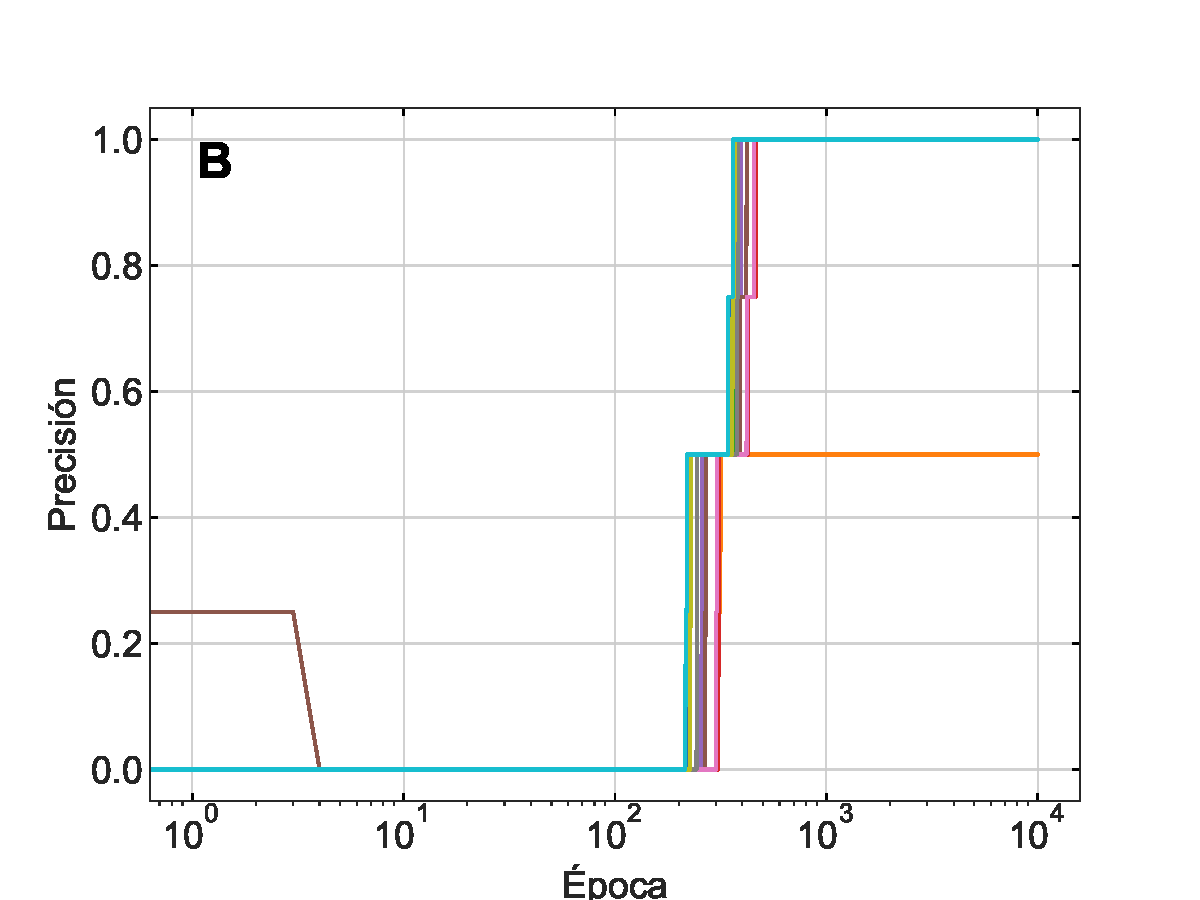
\includegraphics[width=1.1\textwidth]{Figuras/acc_ej1a.pdf}
         \end{subfigure}
         \begin{subfigure}[b]{0.49\linewidth}
            \centering
            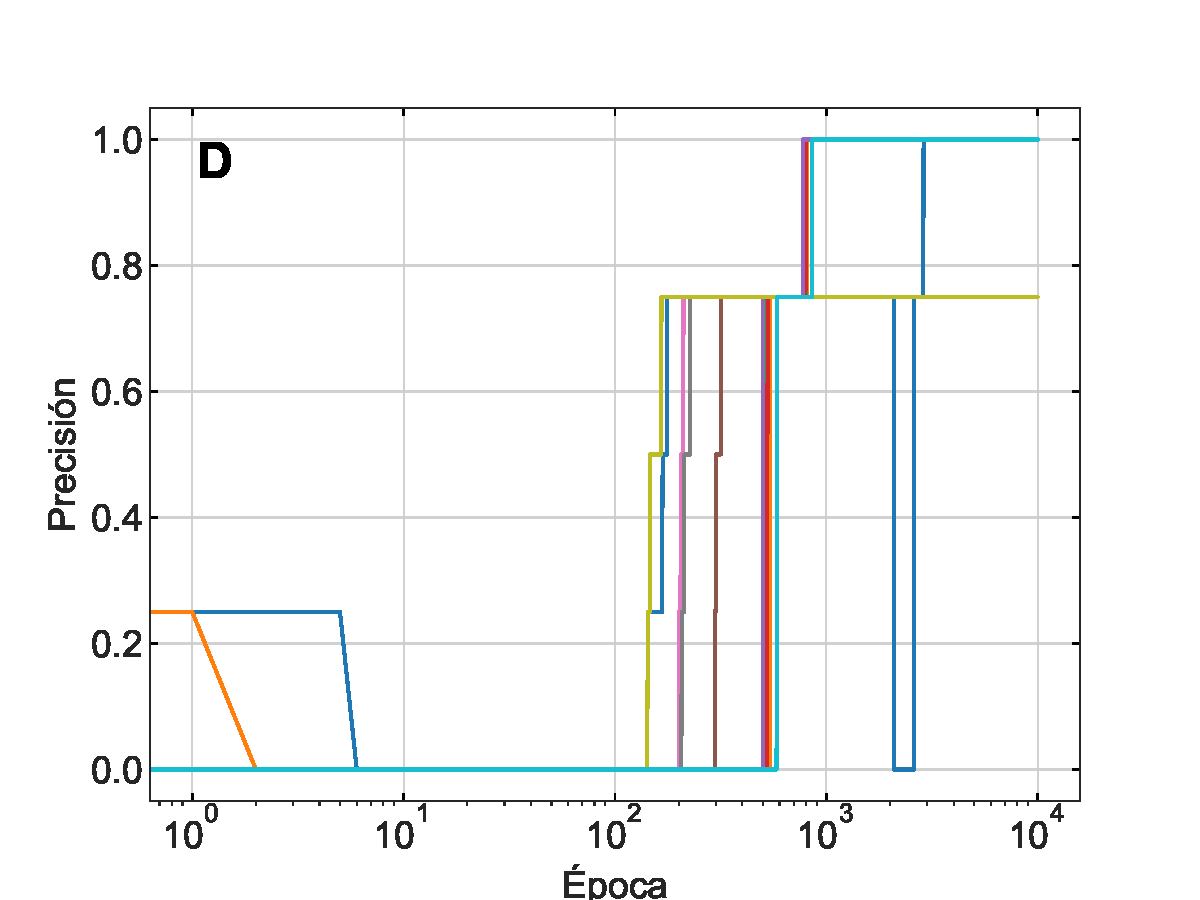
\includegraphics[width=1.1\textwidth]{Figuras/acc_ej1b.pdf}
         \end{subfigure}
    \caption{(A) Error cuadratico medio arquitectura 2-2-1, (B) precisión arquitectura 2-2-1, (C) error cuadratico medio arquitectura 2-1-1 y (D) precisión arquitectura 2-1-1 en función de la época en escala logarítmica para 10 experimentos con distintos pesos iniciales.} 
    \label{fig:1}
\end{figure}

Se definió el tiempo de convergencia para un experimento como la época a partir de la cual el MSE es menor a $0.1$ y este converge a aproximadamente 0 en las 10000 épocas. Es decir para los experimentos que no convergían no se calculó un tiempo de convergencia. Luego, para los experimentos que sí convergían se calculó el tiempo de convergencia promedio obteniendo, para la arquitectura 2-2-1 un tiempo de convergencia de $122.7$ épocas y para la arquitectura 2-1-1 un tiempo de convergencia de $533.33$ épocas. Además se destaca que para la primer arquitectura convergieron\footnote{El término converger se utiliza cuando el MSE, luego del entrenamiento, es aproximadamente 0} 9 de 10 experimentos y para la segunda 6 de 10.

Se promediaron las curvas de precisión y MSE para los 10 experimentos realizados con condiciones iniciales aleatorias para cada arquitectura con el objetivo de comparar la evolución de dichos parámetros en función de las épocas. Los resultados se muestran en la Fig. \ref{fig:1prom}. 

\begin{figure}[h]
    \centering
         \begin{subfigure}[b]{0.49\linewidth}
            \centering
            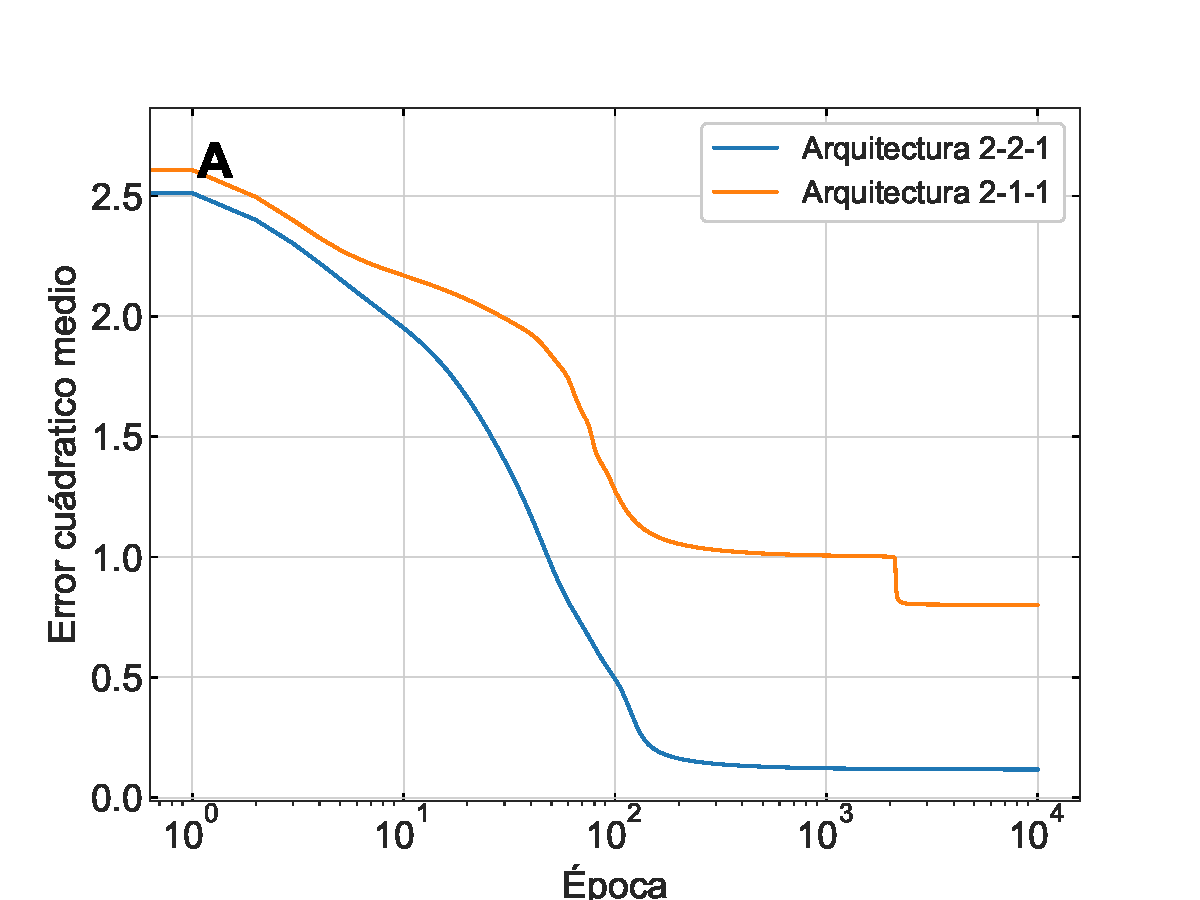
\includegraphics[width=1.1\textwidth]{Figuras/mseprom_ej1.pdf}
         \end{subfigure}
         \begin{subfigure}[b]{0.49\linewidth}
            \centering
            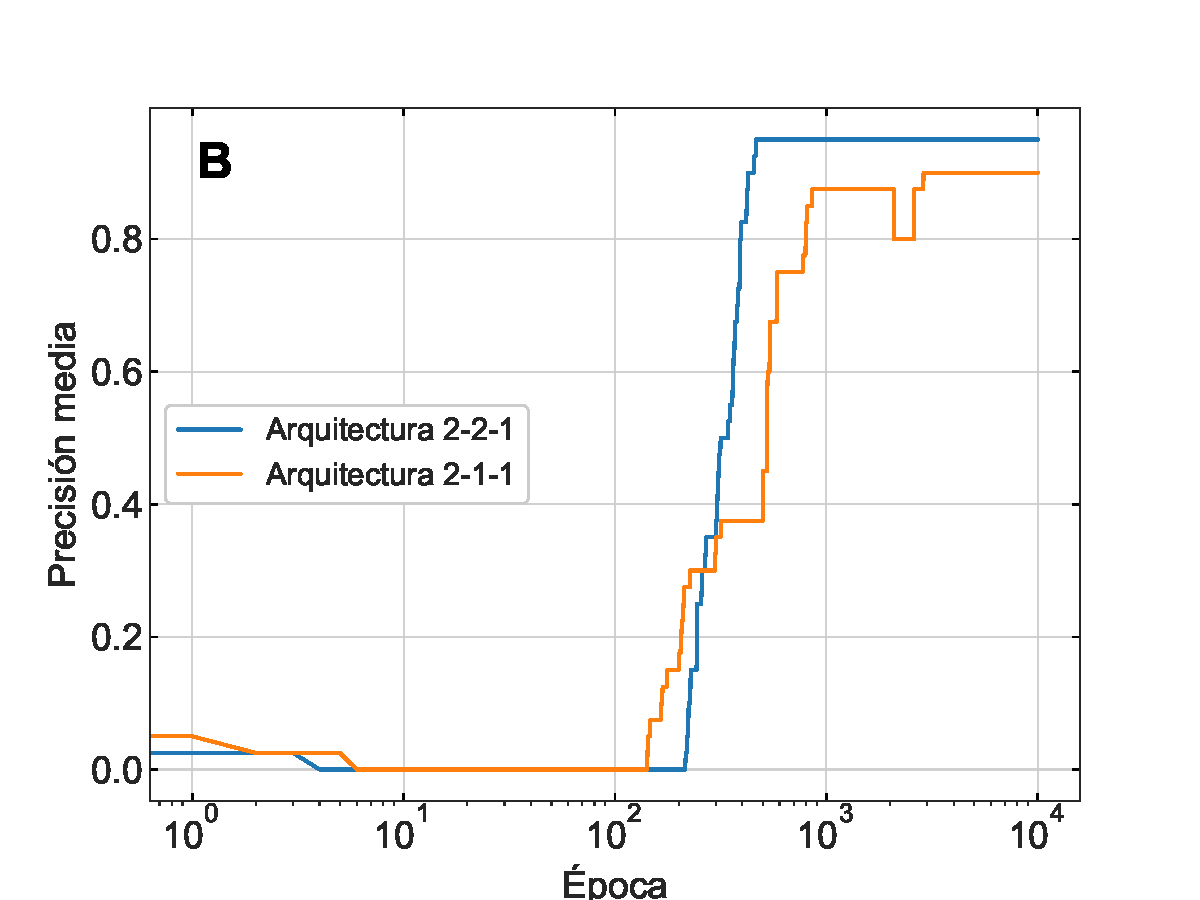
\includegraphics[width=1.1\textwidth]{Figuras/accprom_ej1.pdf}
         \end{subfigure}
    \caption{Arquitectura $2-1-1$. Error cuadratico medio (A) y precisión (B) en función de la época en escala logarítmica para 10 experimentos con distintos pesos iniciales.} 
    \label{fig:1prom}
\end{figure}

Se observa que, luego de 10000 épocas, con la arquitectura 2-2-1 se obtiene una mayor precisión y menor MSE promedio. En resumen, en base a estos resultados, la arquitectura 2-2-1 parece ser la más adecuada para resolver el problema del XOR. No obstante, para ambas arquitecturas el resultado obtenido depende fuertemente de los valores iniciales ya que, por ejemplo, no siempre se obtuvo que la 2-2-1 resuelve 9 de cad 10 casos. También el valor de la tasa de aprendizaje $\eta$ y el número de épocas son parámetros que pueden afectar el aprendizaje de la red.


%\newpage
\section{Aprendizaje del problema de paridad \label{sec:ej2}}

\vspace{0.3cm}

El problema de paridad es una generalización del XOR para una capa de entrada con $N$ neuronas. La salida es $+1$ si el producto de las entradas es $+1$ y $-1$ si el producto de las entradas es $-1$. Mediante el algoritmo de retropropagación se resolvió el problema de paridad utilizando una capa oculta densa con $N'$ neuronas como se muestra en el esquema de la Fig. \ref{fig:esq_2}. 

\begin{figure}[H]
    \centering
         \begin{subfigure}[b]{0.75\linewidth}
            \centering
            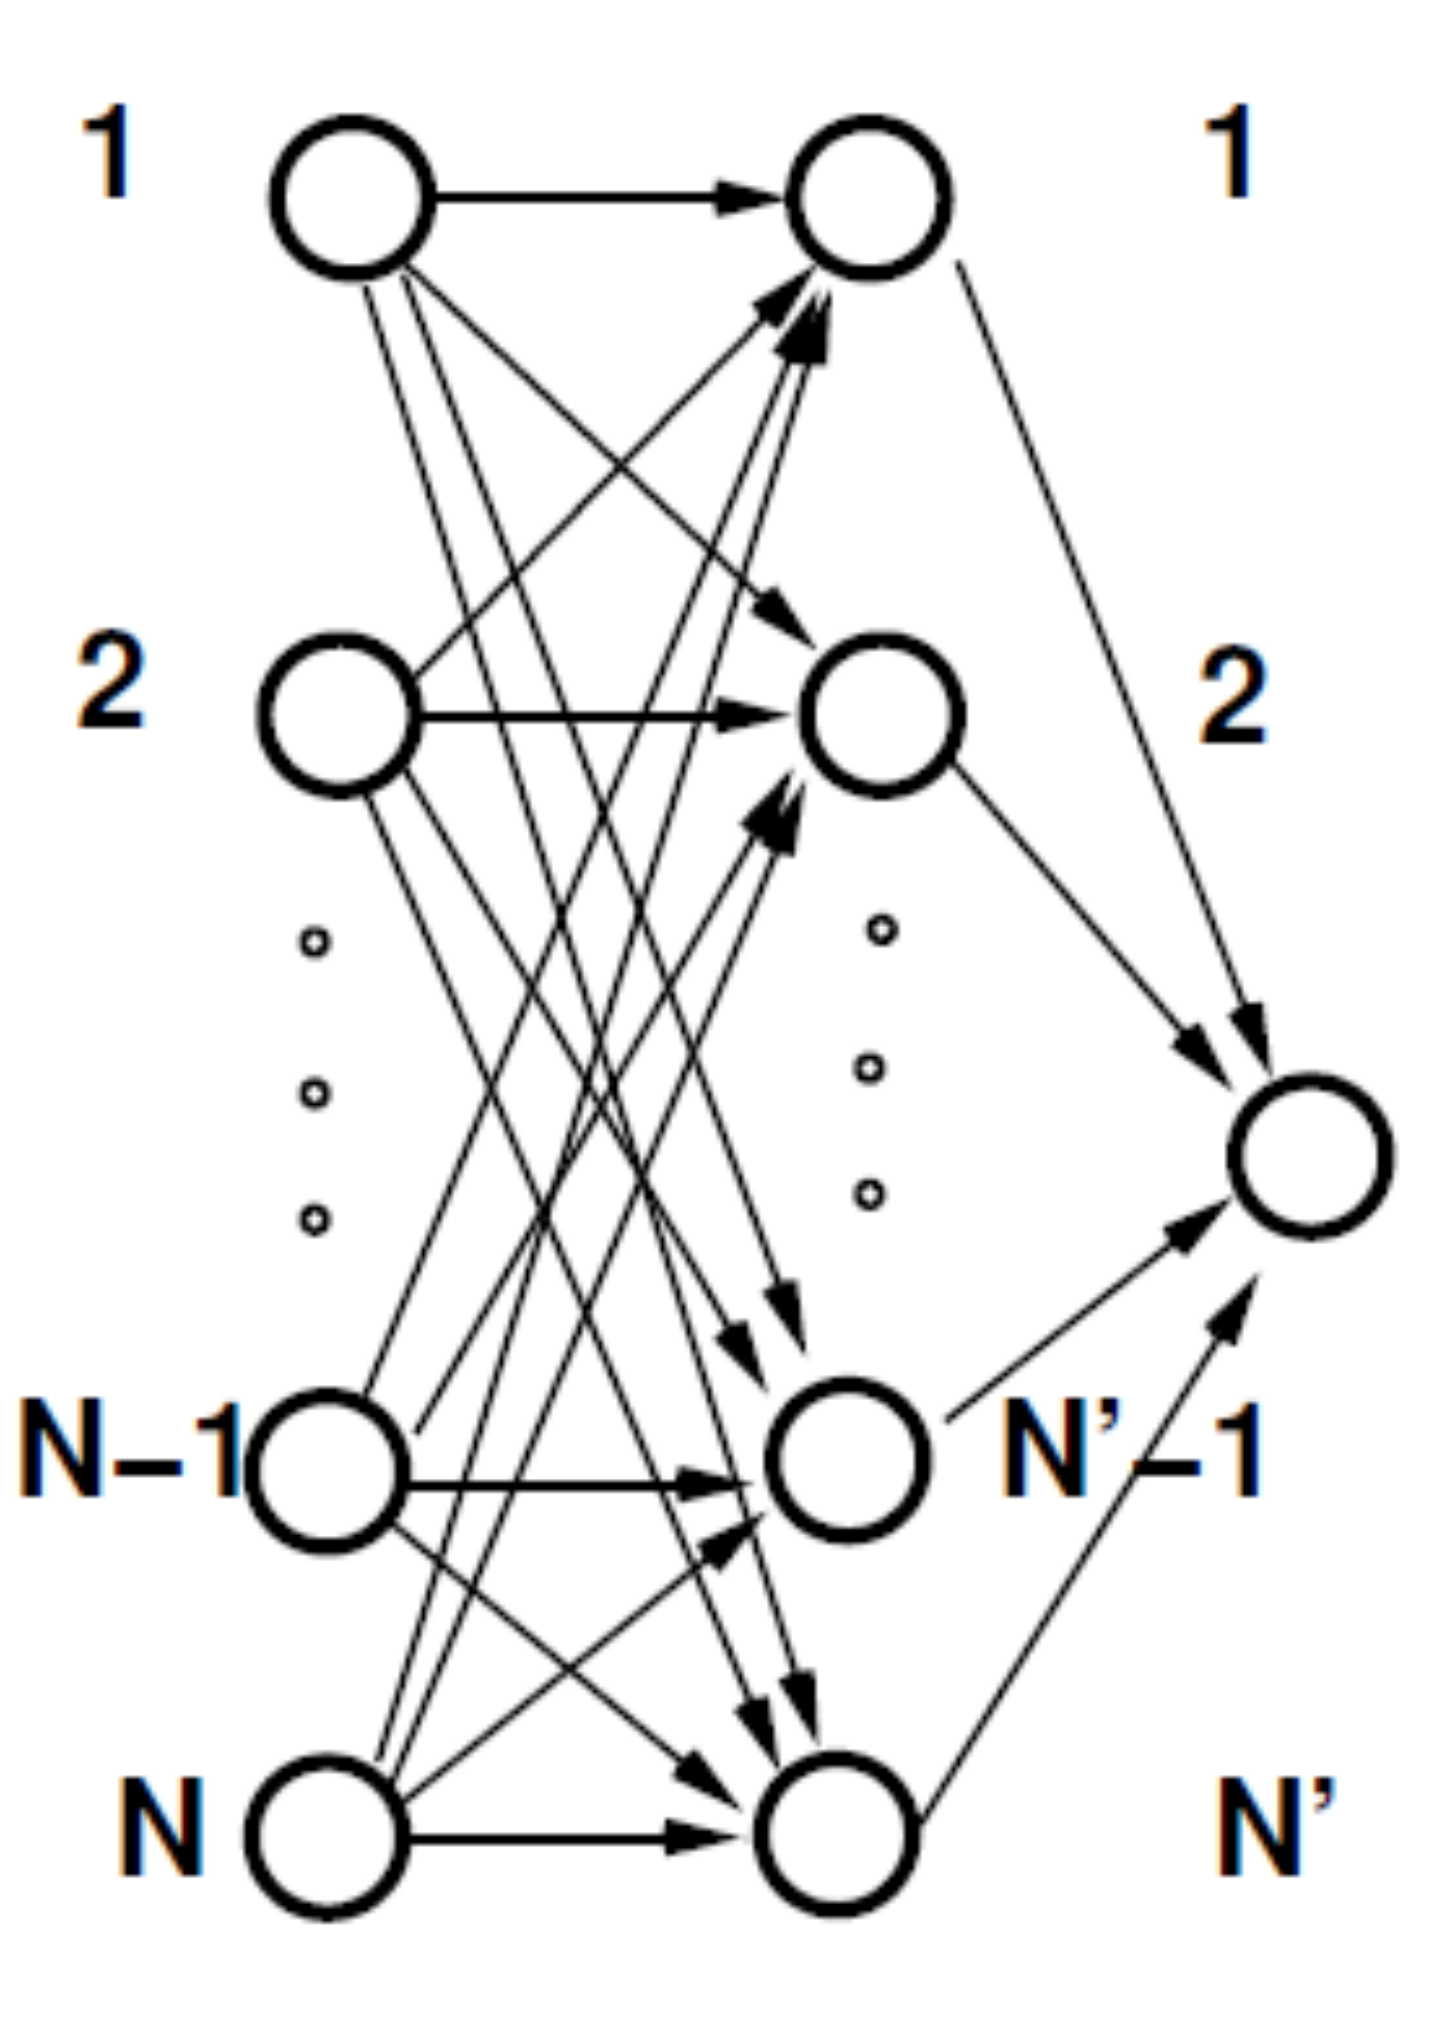
\includegraphics[width=0.5\textwidth]{Figuras/esquema2.png}
         \end{subfigure}
    \caption{Arquitectura de la red neuronal para el problema de paridad.} 
    \label{fig:esq_2}
\end{figure}
\begin{figure}[ht]
    \centering
         \begin{subfigure}[b]{\linewidth}
            \centering
            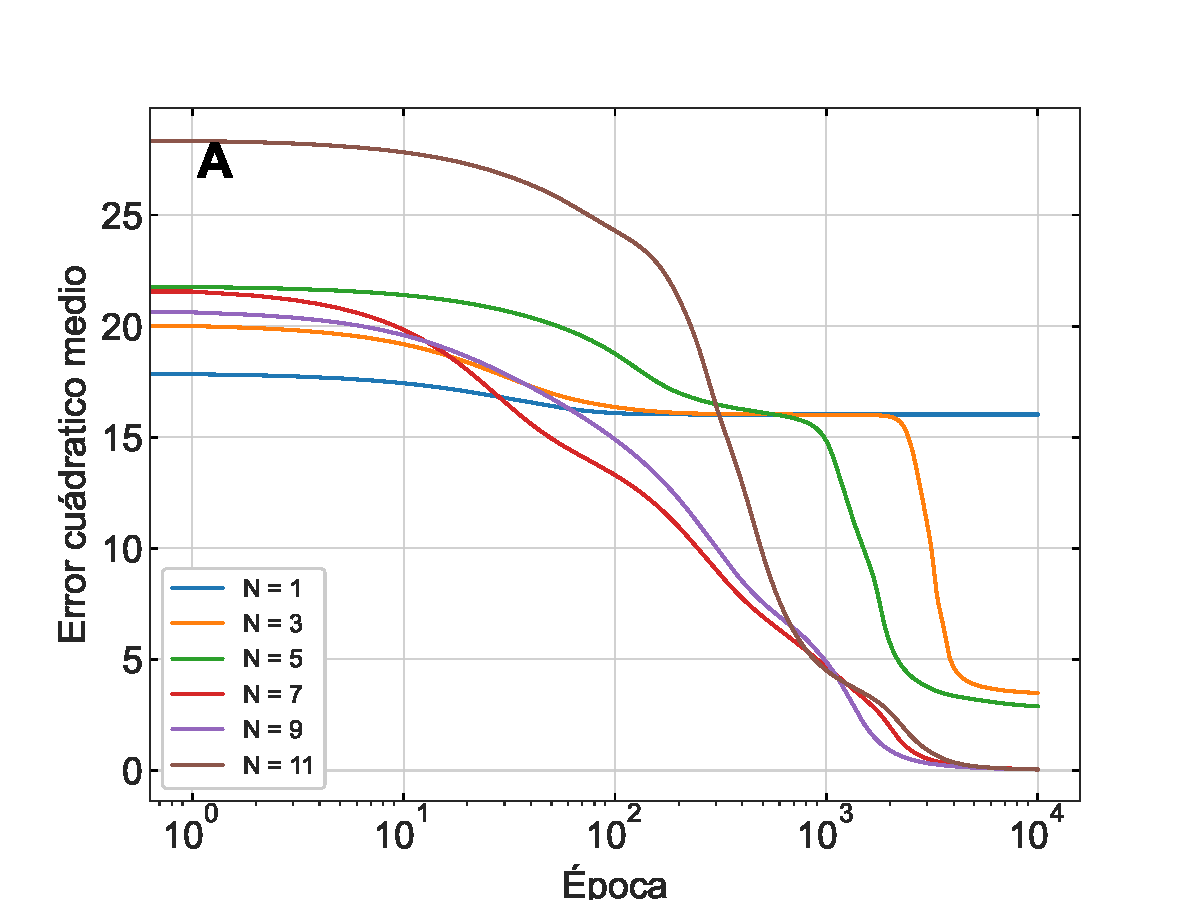
\includegraphics[width=\textwidth]{Figuras/mse_ej2.pdf}
         \end{subfigure}
         \begin{subfigure}[b]{\linewidth}
            \centering
            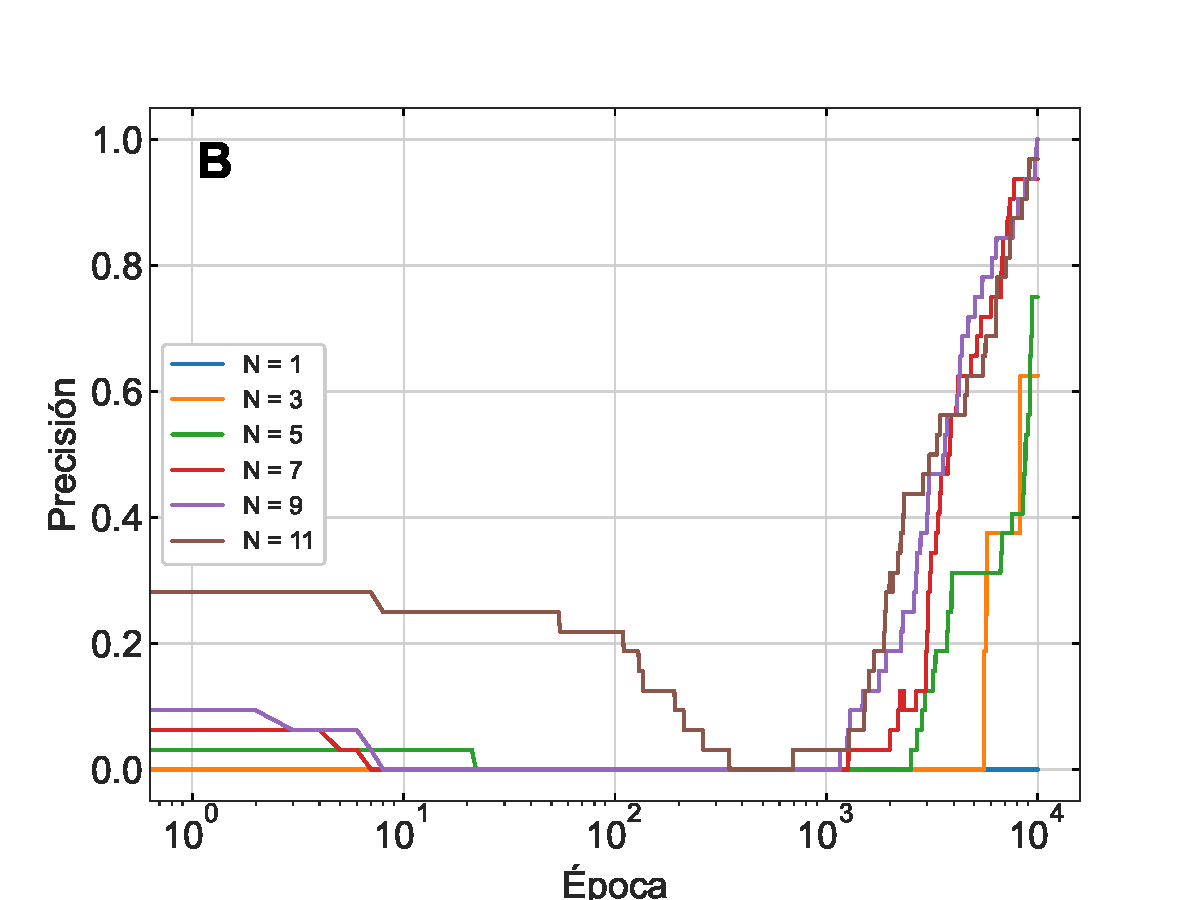
\includegraphics[width=\textwidth]{Figuras/acc_ej2.pdf}
         \end{subfigure}
    \caption{Error cuadratico medio (A) y precisión (B) en función de la época en escala logarítmica para cada número $N' = 1,3,5,7,9,11$ de neuronas en la capa oculta.} 
    \label{fig:2}
\end{figure}

Se realizaron entrenamientos con $N' = 1,3,5,7,9,11$ para estudiar el efecto del aumento de neuronas de la capa oculta en la respuesta de la red. Para el entrenamiento de la red se utilizaron todas las entradas posibles para $N=5$, es decir $2^{N} = 32$ combinaciones de $1$ y $-1$ sin importar el orden. Se utilizó una tasa de aprendizaje de $0.001$ y se entrenó la red durante $10000$ épocas. La evolución del MSE y de la precisión se muestran en las Figs. \ref{fig:2}A y \ref{fig:2}B respectivamente. Se observa como para $N'>N$ la red aprende el problema de paridad con una precisión de aproximadamente el $100\%$ y un MSE de aproximadamente $0$. En cambio, para $N' < N$ la red tiene más problemas para aprender el problema de paridad y que se ve que al disminuir $N'$ la precisión disminuye y el MSE aumenta.

\section{Aprendizaje del mapeo logístico\label{sec:ej3}}

\vspace{0.3cm}

Por último, utilizando el algoritmo de retropropagación se entrenó una red con el objetivo de aprender el mapeo logístico dado por 
\begin{equation}
    x_{n+1} = 4 x_n (1- x_n).
\end{equation}

La arquitectura de la red consistió en una capa oculta densa compuesta de 5 neuronas y una conexión de las neuronas de entrada a la de salida como se muestra en la Fig. \ref{fig:esq_3}. En este caso se utilizó como función de activación de las neuronas de la capa oculta la sigmoidea $g(x) = 1/(1 + \exp{(-x)})$ y la función linel para la neurona de salida. Las neuronas incluyen \textit{bias}.

\begin{figure}[ht]
    \centering
         \begin{subfigure}[b]{0.75\linewidth}
            \centering
            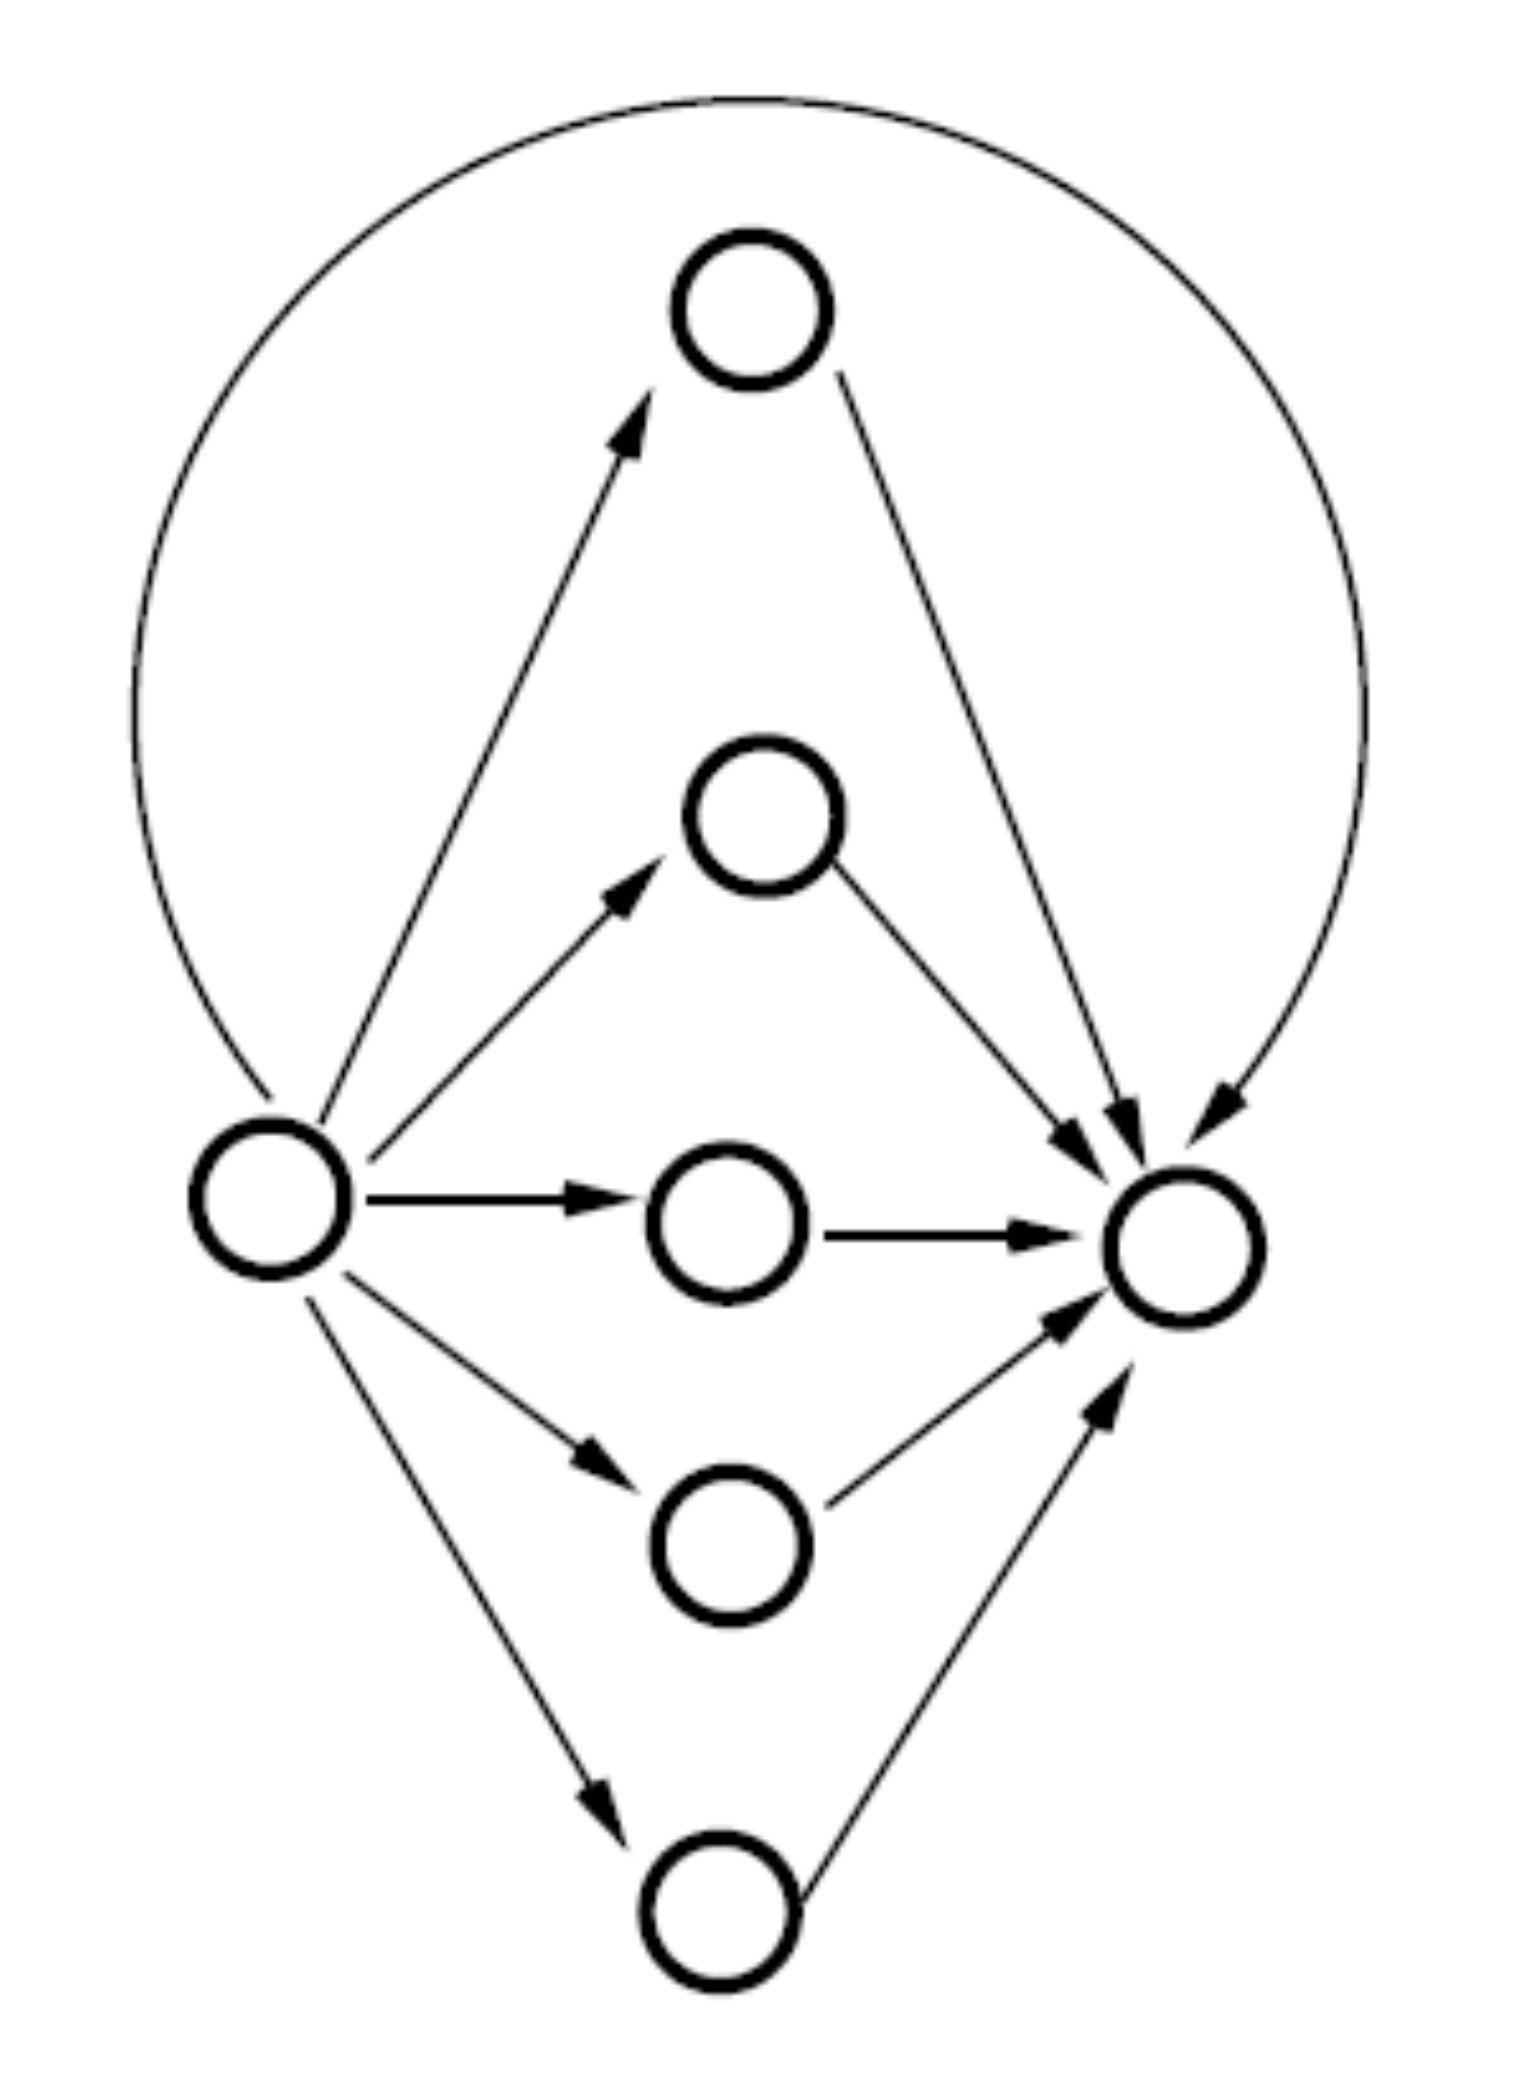
\includegraphics[width=0.5\textwidth]{Figuras/esquema3.png}
         \end{subfigure}
    \caption{Arquitectura de la red neuronal para el aprendizaje del mapeo logístico.} 
    \label{fig:esq_3}
\end{figure}

Se generaron dos bases de datos: Una con $N$ pares de datos $(x_n, x_{n+1})$ para entrenar la red neuronal y otra de $100$ pares para validación de la red. Se implementaron 3 casos para $N=5,10,100$ con el objetivo de estudiar los resultados obtenidos en función de la cantidad de datos de entrenamiento de la red. Se utilizó una tasa de aprendizaje de $0.01$ y se entrenó la red durante $3000$ épocas. La Fig. \ref{fig:mse_3} muestra la evolución del MSE y el error de validación para cada conjunto de ejemplos presentados. 
 
\begin{figure}[ht]
    \centering
         \begin{subfigure}[b]{\linewidth}
            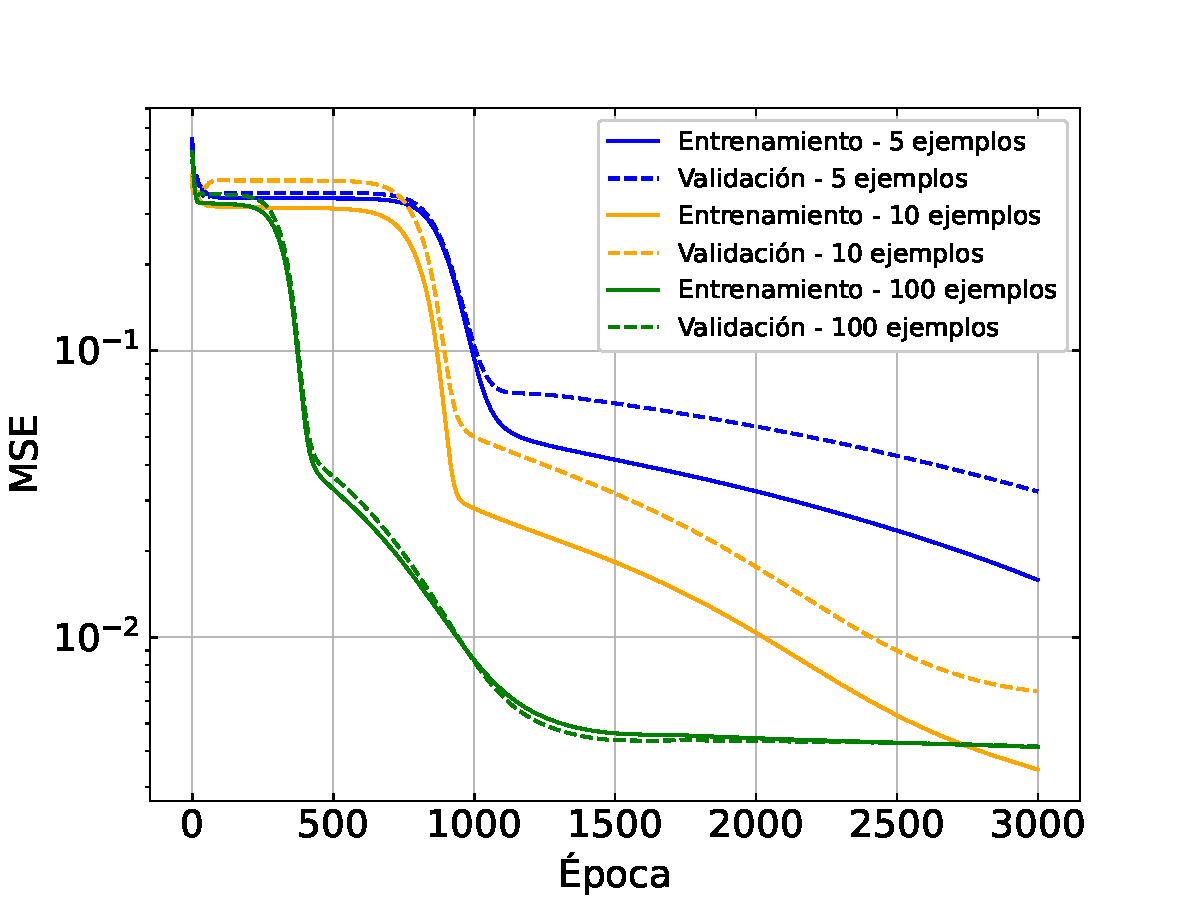
\includegraphics[width=\textwidth]{Figuras/mse_ej3.pdf}
         \end{subfigure}
    \caption{Error cuadrático medio en escala logarítmica del conjunto de entrenamiento y del conjunto de validación en función de la época para $N=5,10,100$ ejemplos del conjunto de entrenamiento.} 
    \label{fig:mse_3}
\end{figure}

\begin{figure*}[ht]
    \centering
         \begin{subfigure}[b]{0.3\linewidth}
            \centering
            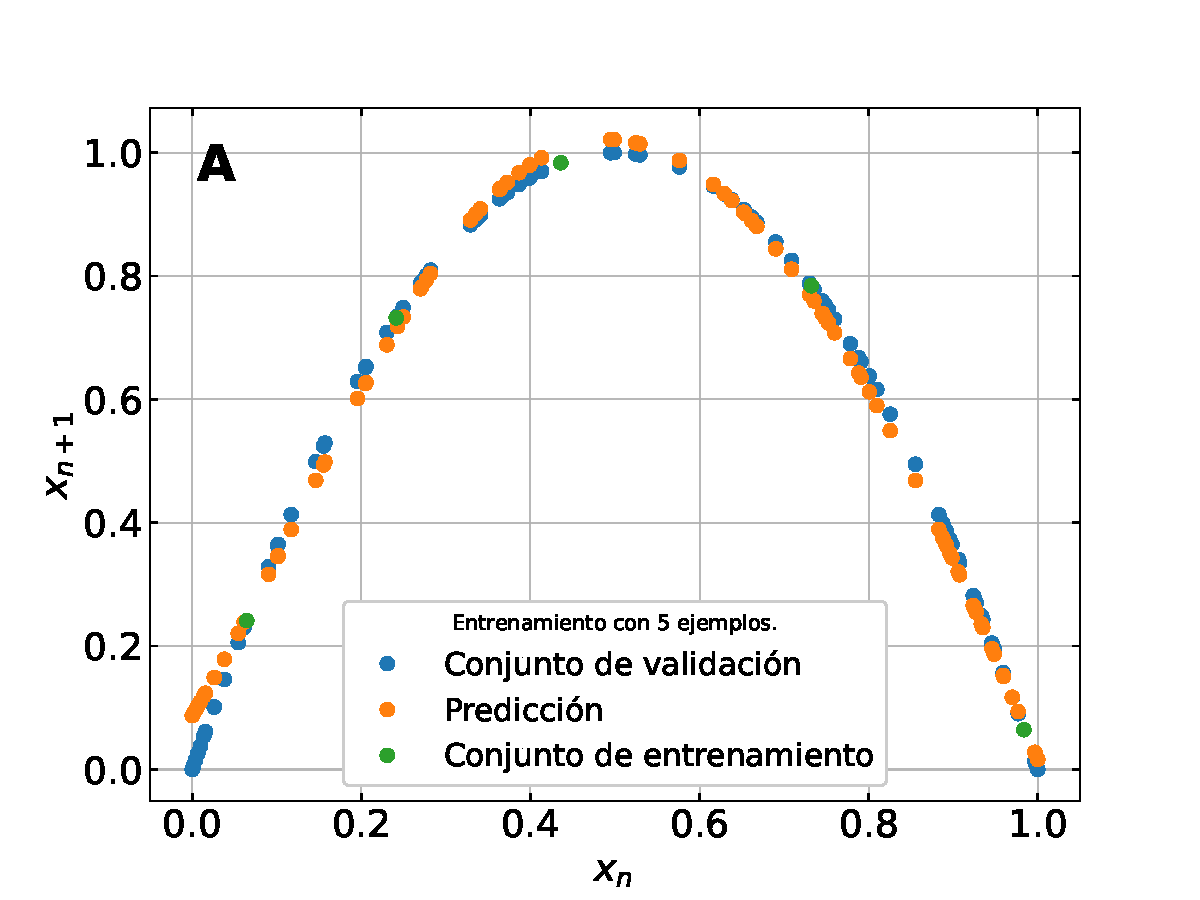
\includegraphics[width=\textwidth]{Figuras/logmap_5_tests_ej3.pdf}
         \end{subfigure}
         \begin{subfigure}[b]{0.3\linewidth}
            \centering
            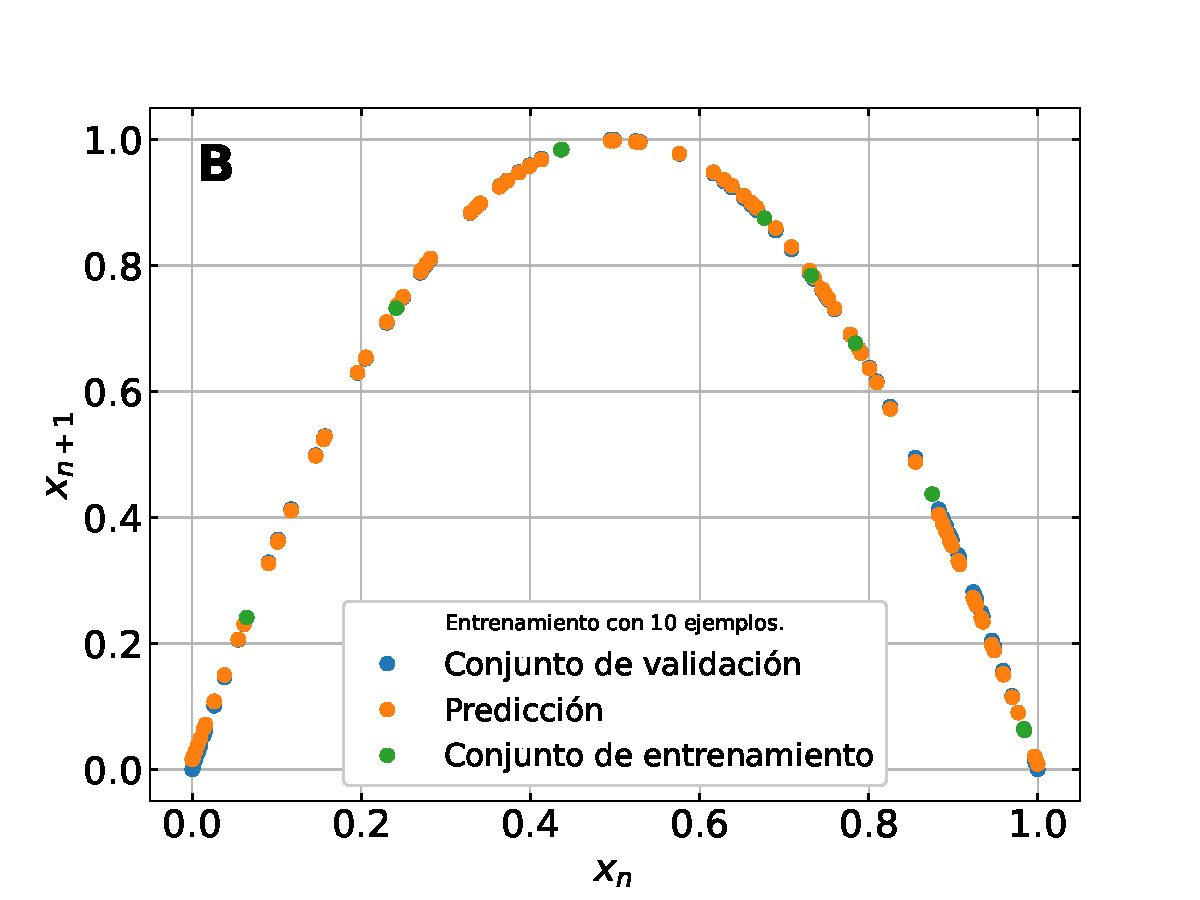
\includegraphics[width=\textwidth]{Figuras/logmap_10_tests_ej3.pdf}
         \end{subfigure}
         \begin{subfigure}[b]{0.3\linewidth}
            \centering
            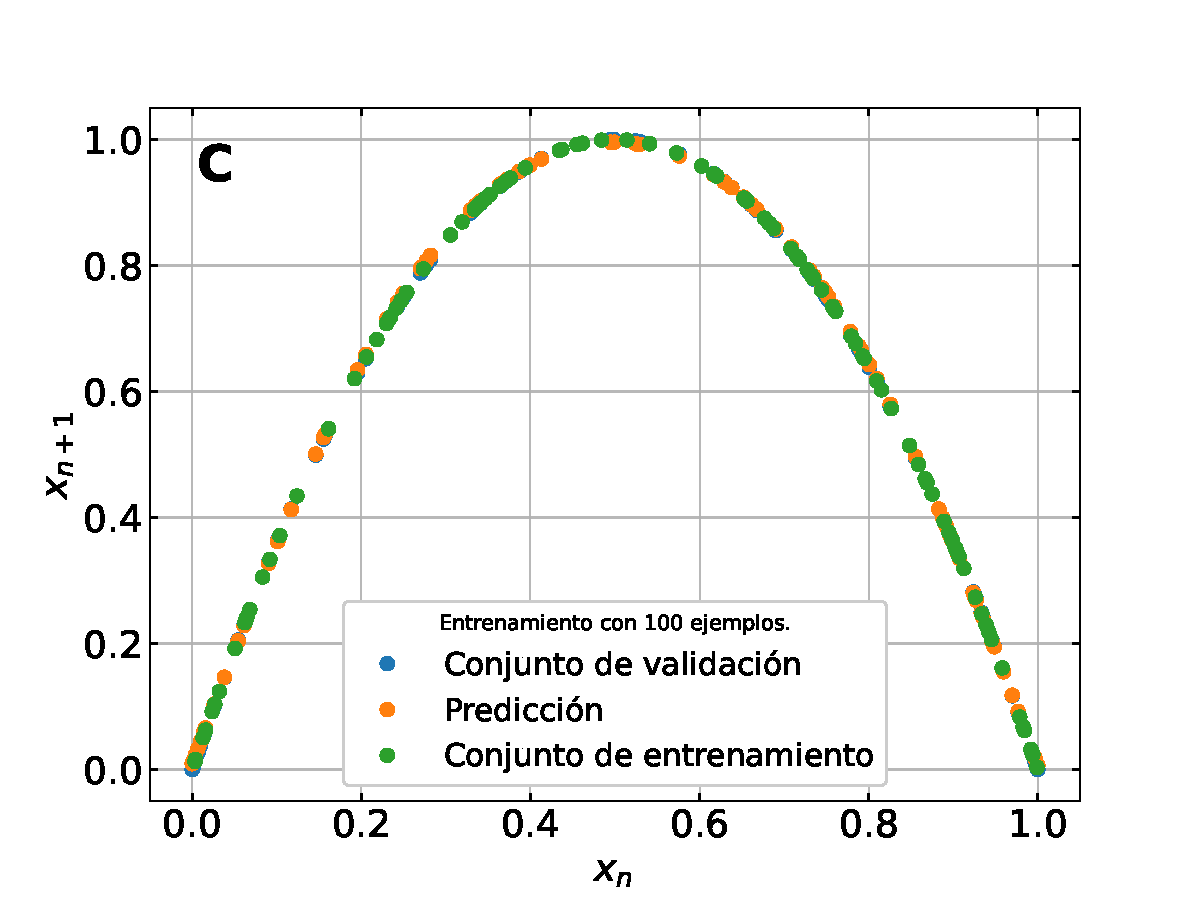
\includegraphics[width=\textwidth]{Figuras/logmap_100_tests_ej3.pdf}
         \end{subfigure}
    \caption{Resultados obtenidos para el aprendizaje del mapeo logístico para $N=5,10,100$ ejemplos del conjunto de entrenamiento. Se muestra el conjunto de validación ($N$ ejemplos), el conjunto de entrenamiento y la predicción de la red (100 datos).} 
    \label{fig:logmap_3}
\end{figure*}
En primer lugar, para todos los casos notamos que el error de validación es siempre mayor al del de entrenamiento. Para $N = 5,10$ podemos ver que a partir de una dada época, las curvas del MSE del conjunto de entrenamiento y del conjunto de validación se separan y el MSE del entrenamiento sigue disminuyendo mientras el MSE del conjunto de validación no. Esto indica que la red encuentra un conjunto de pesos que le permite resolver los casos de entrenamiento adecuadamente pero esto no resuelve el problema del mapeo logístico de forma general. Para $N=100$ las curvas no se despegan en todo el entrenamiento y el error de entrenamiento y de validación luego del entrenamiento son un orden de magnitud menor en comparación a los casos $N = 5,10$. La Fig. \ref{fig:logmap_3} muestra la comparación entre la predicción de la red para el mapeo logístico y el conjunto de validación, para $N=5,10,100$ ejemplos del conjunto de entrenamiento. Se observa que para $N=5$ la predicción de la red no es del todo adecuada, especialmente lejos de los valores de entrenamiento ya que cerca de los mismos la predicción si buena. Para $N=10$ la predicción de la red es mejor que para $N=5$ pero al igual que antes se aleja en zonas sin valores de entrenamiento. Para $N=100$ la predicción de la red es muy buena y se superpone con el conjunto de validación. 



% Bibliography
%\renewcommand*{\bibfont}{\normalsize}
%\bibliography{Redes}

% Full bibliography added automatically for Optics Letters submissions; the following line will simply be ignored if submitting to other journals.
% Note that this extra page will not count against page length
%\bibliographyfullrefs{Redes}


\centerline{\rule{0.95\linewidth}{0.6pt}}

\clearpage

\begin{onecolumn} % Activa una sola columna para el apéndice
\appendix
\section{Apéndice \label{codigo}}

\begin{lstlisting}[language=Python, caption={Ejercicio 1 - Arquitectura 2-2-1}, label=ej1]

import numpy as np
import matplotlib.pyplot as plt

#Ploteo 
import seaborn as sns
#sns.axes_style("whitegrid")
sns.set_style("ticks")

# Funcion de activacion
def act(x):
    return np.tanh(x)
def dact(x):
    return 1 - np.tanh(x) ** 2
# Funcion de coste (error cuadratico medio)
def mse_loss(y, O):
    E = (y - O) ** 2
    return 0.5*np.sum(E)

# Datos de entrada y salida para XOR
x_train = np.array([[-1, -1], [-1, 1], [1, -1], [1, 1]])  # Entradas
y_train = np.array([[-1], [1], [1], [-1]])  # Salidas

#Arquitectura de la red
input_size = 2
hidden_size = 2
output_size = 1
learning_rate = 0.05
num_epochs = 10000
epochs = [i for i in range(0, num_epochs)]
num_exps = 10
num_test = len(x_train)

fig1, ax1 = plt.subplots(figsize=(8,6)) 
fig2, ax2 = plt.subplots(figsize=(8,6)) 
fig3, ax3 = plt.subplots(figsize=(8,6)) 
fig4, ax4 = plt.subplots(figsize=(8,6)) 

loss_prom = np.zeros(num_epochs)
accs_prom = np.zeros(num_epochs)
epochs_prom = []
epoch_aux = 0

for n in range(num_exps):
    print("Experimento numero: ", n)
    loss = np.zeros(num_epochs)
    accs = np.zeros(num_epochs)

    # Pesos iniciales aleatorios
    w = np.random.uniform(-1,1,size=(hidden_size, input_size))   #filas #columnas
    W = np.random.uniform(-1,1,size=(output_size, hidden_size)) 
    b1 = np.random.uniform(-1,1,size=(1,hidden_size)).reshape(-1, 1)
    b2 = np.random.uniform(-1,1,size=(1,output_size)).reshape(-1, 1) 

    for epoch in epochs:
        #print("epoch",epoch)
        acc = 0  
        for u in range(num_test):

            x = x_train[u].reshape(-1, 1)
            y = y_train[u].reshape(-1, 1)

            # Forward propagation
            h1 = np.dot(w, x) + b1 #input de la capa oculta
            V = act(h1) #output de la capa oculta
            h2 = np.dot(W, V) + b2 #input de la capa de salida
            O = act(h2) #output de la capa de salida

            # Calculo de la perdida
            loss[epoch] += mse_loss(y, O)
            loss_prom[epoch] += mse_loss(y, O)

            #Calculo de la precision 
    
            if(abs(O - y) < 0.1*abs(y)):
                acc += 1

            # Backpropagation
            delta2 = dact(h2)*(y-O)
            delta1 = dact(h1)*np.dot(W.T,delta2)

            # Actualizacion de pesos
            W += learning_rate*np.dot(delta2, V.T) 
            b2 += learning_rate*delta2*(1) 
            w += learning_rate*np.dot(delta1, x.T) 
            b1 += learning_rate*delta1*(1) 

            #if (epoch == num_epochs-1):
                #print("Output ", O)
                #print("W ", W)
                #print("w ", w)
        
        accs[epoch] += acc/num_test
        accs_prom[epoch] += acc/num_test

        #if epoch % 500 == 0:
        #    print(f'Epoch {epoch}: Loss = {loss[epoch]}')

    found_epoch = False
    for epoch in range(num_epochs-1, -1, -1):
        if (loss[epoch] > 0.1 and not found_epoch):
            epoch_aux = epoch
            found_epoch = True
        if found_epoch:
            break
    if(loss[-1] < 0.1):
        epochs_prom.append(epoch_aux)

    print("Entrenamiento " + str(n) + " completado.")

    ax1.semilogx(epochs, loss, "-")
    ax1.set_xlabel(r"Epoca", fontsize=18)
    ax1.set_ylabel(r"Error cuadratico medio", fontsize=18)
    ax1.tick_params(direction='in', top=True, right=True, left=True, bottom=True)
    ax1.tick_params(axis='x', rotation=0, labelsize=18, color='black')
    ax1.tick_params(axis='y', labelsize=18, color='black')
    #ax1.set_xlim(0, 10000)
    ax1.text(0.05, 0.95, r'A' , transform=ax1.transAxes, fontsize=24,
     verticalalignment='top', fontweight='bold', color="black")
    ax1.grid(True, linewidth=0.5, linestyle='-', alpha=0.9)
    fig1.savefig(f"../Redes-Neuronales/Practica_4/resultados/ej1a/mse_ej1a.pdf")
    fig1.savefig(f"../Redes-Neuronales/Practica_4/resultados/ej1a/mse_ej1a.png",
     dpi=600)
    ax2.semilogx(epochs, accs, "-")
    ax2.set_xlabel(r"Epoca", fontsize=18)
    ax2.set_ylabel(r"Precision", fontsize=18)
    ax2.tick_params(direction='in', top=True, right=True, left=True, bottom=True)
    ax2.tick_params(axis='x', rotation=0, labelsize=18, color='black')
    ax2.tick_params(axis='y', labelsize=18, color='black')
    #ax2.set_xlim(0, 10000)
    ax2.text(0.05, 0.95, r'B' , transform=ax2.transAxes, fontsize=24, 
    verticalalignment='top', fontweight='bold', color="black")
    ax2.grid(True, linewidth=0.5, linestyle='-', alpha=0.9)
    fig2.savefig(f"../Redes-Neuronales/Practica_4/resultados/ej1a/acc_ej1a.pdf")
    fig2.savefig(f"../Redes-Neuronales/Practica_4/resultados/ej1a/acc_ej1a.png",
     dpi=600)

print(epochs_prom)
print("Epoca de convergencia", np.mean(epochs_prom))

loss_prom = loss_prom/num_exps
accs_prom = accs_prom/num_exps

if len(epochs) == len(loss_prom) == len(accs_prom):
    # Combina los arrays en una sola matriz
    data = np.column_stack((epochs, loss_prom, accs_prom))

    # Especifica el nombre de archivo en el que deseas guardar los datos
    file_name = "../Redes-Neuronales/Practica_4/resultados/ej1a/prom_ej1a.txt"

    # Guarda los datos en el archivo de texto
    np.savetxt(file_name, data, fmt="%d %.6f %.6f")
\end{lstlisting}
\begin{lstlisting}[language=Python, caption={Ejercicio 1 - Arquitectura 2-1-1}, label=ej1b]

import numpy as np
import matplotlib.pyplot as plt

#Ploteo 
import seaborn as sns
#sns.axes_style("whitegrid")
sns.set_style("ticks")

# Funcion de activacion
def act(x):
    return np.tanh(x)
def dact(x):
    return 1 - np.tanh(x) ** 2
# Funcion de coste (error cuadratico medio)
def mse_loss(y, O):
    E = (y - O) ** 2
    return 0.5*np.sum(E)

# Datos de entrada y salida para XOR
x_train = np.array([[-1, -1], [-1, 1], [1, -1], [1, 1]])  # Entradas
y_train = np.array([[-1], [1], [1], [-1]])  # Salidas

#Arquitectura de la red
input_size = 2
hidden_size = 1
output_size = 1
learning_rate = 0.05
num_epochs = 10000
epochs = [i for i in range(0, num_epochs)]
num_exps = 10
num_test = len(x_train)

fig1, ax1 = plt.subplots(figsize=(8,6)) 
fig2, ax2 = plt.subplots(figsize=(8,6)) 
fig3, ax3 = plt.subplots(figsize=(8,6)) 
fig4, ax4 = plt.subplots(figsize=(8,6)) 

loss_prom = np.zeros(num_epochs)
accs_prom = np.zeros(num_epochs)
epochs_prom = []
epoch_aux = 0

for n in range(num_exps):
    print("Experimento numero: ", n)
    loss = np.zeros(num_epochs)
    accs = np.zeros(num_epochs)

    # Pesos iniciales aleatorios
    w = np.random.uniform(-1,1,size=(hidden_size, input_size)) #filas #columnas
    W = np.random.uniform(-1,1,size=(output_size, hidden_size + input_size))
    b1 = np.random.uniform(-1,1,size=(1,hidden_size)).reshape(-1, 1) 
    b2 = np.random.uniform(-1,1,size=(1,output_size)).reshape(-1, 1) 

    for epoch in epochs:
        #print("epoch",epoch)
        acc = 0  
        for u in range(num_test):

            x = x_train[u].reshape(-1, 1)
            y = y_train[u].reshape(-1, 1)

            # Forward propagation
            h1 = np.dot(w, x) + b1 #input de la capa oculta
            V = act(h1) #output de la capa oculta
            concatenate = np.vstack((V, x)) 
            h2 = np.dot(W,concatenate) + b2 #input de la capa de salida
            O = act(h2) #output de la capa de salida

            # Calculo de la perdida
            loss[epoch] += mse_loss(y, O)
            loss_prom[epoch] += mse_loss(y, O)

            #Calculo de la precision 
    
            if(abs(O - y) < 0.1*abs(y)):
                acc += 1

            # Backpropagation
            delta2 = dact(h2)*(y-O)
            delta1 = dact(h1)*np.dot(W[:, :hidden_size].T,delta2)

            # Actualizacion de pesos
            W += learning_rate*np.dot(delta2, concatenate.T) 
            b2 += learning_rate*delta2*(1) 
            w += learning_rate*np.dot(delta1, x.T) 
            b1 += learning_rate*delta1*(1) 

            #if epoch == num_epochs-1:
                #print("Output ", O)
                #print("W ", W)
                #print("w ", w)
    
        accs[epoch] += acc/num_test
        accs_prom[epoch] += acc/num_test

        #if epoch % 500 == 0:
        #    print(f'Epoch {epoch}: Loss = {loss[epoch]}')
    
    found_epoch = False
    for epoch in range(num_epochs-1, -1, -1):
        if (loss[epoch] > 0.1 and not found_epoch):
            epoch_aux = epoch
            found_epoch = True
        if found_epoch:
            break
    if(loss[-1] < 0.1):
        epochs_prom.append(epoch_aux)
    
    print("Entrenamiento " + str(n) + " completado.")

    ax1.semilogx(epochs, loss, "-")
    ax1.set_xlabel(r"Epoca", fontsize=18)
    ax1.set_ylabel(r"Error cuadratico medio", fontsize=18)
    ax1.tick_params(direction='in', top=True, right=True, left=True, bottom=True)
    ax1.tick_params(axis='x', rotation=0, labelsize=18, color='black')
    ax1.tick_params(axis='y', labelsize=18, color='black')
    #ax1.set_xlim(0, 10000)
    ax1.text(0.05, 0.95, r'C' , transform=ax1.transAxes, fontsize=24,
     verticalalignment='top', fontweight='bold', color="black")
    ax1.grid(True, linewidth=0.5, linestyle='-', alpha=0.9)
    fig1.savefig(f"../Redes-Neuronales/Practica_4/resultados/ej1b/mse_ej1b.pdf")
    fig1.savefig(f"../Redes-Neuronales/Practica_4/resultados/ej1b/mse_ej1b.png",
     dpi=600)

    ax2.semilogx(epochs, accs, "-")
    ax2.set_xlabel(r"Epoca", fontsize=18)
    ax2.set_ylabel(r"Precision", fontsize=18)
    ax2.tick_params(direction='in', top=True, right=True, left=True, bottom=True)
    ax2.tick_params(axis='x', rotation=0, labelsize=18, color='black')
    ax2.tick_params(axis='y', labelsize=18, color='black')
    #ax2.set_xlim(0, 10000)
    ax2.text(0.05, 0.95, r'D' , transform=ax2.transAxes, fontsize=24, 
    verticalalignment='top', fontweight='bold', color="black")
    ax2.grid(True, linewidth=0.5, linestyle='-', alpha=0.9)
    fig2.savefig(f"../Redes-Neuronales/Practica_4/resultados/ej1b/acc_ej1b.pdf")
    fig2.savefig(f"../Redes-Neuronales/Practica_4/resultados/ej1b/acc_ej1b.png", 
    dpi=600)

loss_prom = loss_prom/num_exps
accs_prom = accs_prom/num_exps

print(epochs_prom)
print("Epoca de convergencia", np.mean(epochs_prom))

if len(epochs) == len(loss_prom) == len(accs_prom):
    # Combina los arrays en una sola matriz
    data = np.column_stack((epochs, loss_prom, accs_prom))

    # Especifica el nombre de archivo en el que deseas guardar los datos
    file_name = "../Redes-Neuronales/Practica_4/resultados/ej1b/prom_ej1b.txt"

    # Guarda los datos en el archivo de texto
    np.savetxt(file_name, data, fmt="%d %.6f %.6f")


\end{lstlisting}

\begin{lstlisting}[language=Python, caption={Ejercicio 2}, label=ej2]

import numpy as np
import matplotlib.pyplot as plt

#Ploteo 
import seaborn as sns
#sns.axes_style("whitegrid")
sns.set_style("ticks")

# Funcion de activacion
def act(x):
    return np.tanh(x)
def dact(x):
    return 1 - np.tanh(x) ** 2
# Funcion de coste (error cuadratico medio)
def mse_loss(y, O):
    E = (y - O) ** 2
    return 0.5*np.sum(E)

# Datos de entrada y salida para XOR generalizado 
import itertools
def generate_input(length):
    # Genera todas las combinaciones posibles de 1 y -1 con la longitud deseada
    combinations = list(itertools.product([1, -1], repeat=length))
    x = np.array(combinations)
    y = np.prod(x, axis=1)
    return x, y
N = 5
x_train, y_train = generate_input(N)

#Arquitectura de la red
input_size = N
hidden_sizes = [1,3,5,7,9,11]
output_size = 1
learning_rate = 0.001
num_epochs = 10000
epochs = [i for i in range(0, num_epochs)]
num_exps = 10
num_test = len(x_train)

fig1, ax1 = plt.subplots(figsize=(8,6)) 
fig2, ax2 = plt.subplots(figsize=(8,6)) 
n=1
for hidden_size in hidden_sizes:
    print("Experimento numero: ", n)
    loss = np.zeros(num_epochs)
    accs = np.zeros(num_epochs)

    # Pesos iniciales aleatorios
    w = np.random.uniform(-1,1,size=(hidden_size, input_size)) #filas #columnas
    W = np.random.uniform(-1,1,size=(output_size, hidden_size)) 
    b1 = np.random.uniform(-1,1,size=(1,hidden_size)).reshape(-1, 1) 
    b2 = np.random.uniform(-1,1,size=(1,output_size)).reshape(-1, 1)

    for epoch in epochs:
        #print("epoch",epoch)
        acc = 0  
        for u in range(num_test):

            x = x_train[u].reshape(-1, 1)
            y = y_train[u].reshape(-1, 1)

            # Forward propagation
            h1 = np.dot(w, x) + b1 #input de la capa oculta
            V = act(h1) #output de la capa oculta
            h2 = np.dot(W, V) + b2 #input de la capa de salida
            O = act(h2) #output de la capa de salida

            # Calculo de la perdida
            loss[epoch] += mse_loss(y, O)
        
            #Calculo de la precision 
    
            if(abs(O - y) < 0.1*abs(y)):
                acc += 1
            accs[epoch] = acc/num_test
                
            # Backpropagation
            delta2 = dact(h2)*(y-O)
            delta1 = dact(h1)*np.dot(W.T,delta2)

            # Actualizacion de pesos
            W += learning_rate*np.dot(delta2, V.T) 
            b2 += learning_rate*delta2*(1) 
            w += learning_rate*np.dot(delta1, x.T) 
            b1 += learning_rate*delta1*(1) 

            #if epoch == num_epochs-1:
                #print("Output ", O)
                #print("W ", W)
                #print("w ", w)

        if epoch % 500 == 0:
            print(f'Epoch {epoch}: Loss = {loss[epoch]}')

    n += 1

    print("Entrenamiento completado.")

    ax1.semilogx(epochs, loss, "-", label = "N = " + str(hidden_size))
    ax1.set_xlabel(r"Epoca", fontsize=18)
    ax1.set_ylabel(r"Error cuadratico medio", fontsize=18)
    ax1.tick_params(direction='in', top=True, right=True, left=True, bottom=True)
    ax1.tick_params(axis='x', rotation=0, labelsize=18, color='black')
    ax1.tick_params(axis='y', labelsize=18, color='black')
    ax1.legend(fontsize=12, framealpha=1, loc = "lower left")
    #ax1.set_xlim(0, 10000)
    ax1.text(0.05, 0.95, r'A' , transform=ax1.transAxes, fontsize=24, 
    verticalalignment='top', fontweight='bold', color="black")
    ax1.grid(True, linewidth=0.5, linestyle='-', alpha=0.9)
    fig1.savefig(f"../Redes-Neuronales/Practica_4/resultados/ej2/mse_ej2.pdf")
    fig1.savefig(f"../Redes-Neuronales/Practica_4/resultados/ej2/mse_ej2.png", 
    dpi=600)

    ax2.semilogx(epochs, accs, "-", label = "N = " + str(hidden_size))
    ax2.set_xlabel(r"Epoca", fontsize=18)
    ax2.set_ylabel(r"Precision", fontsize=18)
    ax2.tick_params(direction='in', top=True, right=True, left=True, bottom=True)
    ax2.tick_params(axis='x', rotation=0, labelsize=18, color='black')
    ax2.tick_params(axis='y', labelsize=18, color='black')
    ax2.legend(fontsize=12, framealpha=1, loc = "center left")
    ax2.text(0.05, 0.95, r'B' , transform=ax2.transAxes, fontsize=24, 
    verticalalignment='top', fontweight='bold', color="black")
    #ax2.set_xlim(0, 10000)
    ax2.grid(True, linewidth=0.5, linestyle='-', alpha=0.9)
    fig2.savefig(f"../Redes-Neuronales/Practica_4/resultados/ej2/acc_ej2.pdf")
    fig2.savefig(f"../Redes-Neuronales/Practica_4/resultados/ej2/acc_ej2.png", 
    dpi=600)

\end{lstlisting}

\begin{lstlisting}[language=Python, caption={Ejercicio 3}, label=ej3]

import tensorflow as tf
import numpy as np
import matplotlib.pyplot as plt

def logistic_map(n):
    x = np.zeros(n+1)
    x[0] = np.random.random()
    for i in range(n):
        x[i+1] = 4 * x[i] * (1 - x[i])
    y = x[1:]
    x = x[:-1]
    return x, y

ntrains = [5,10,100]
ntest = 100
epochs = 3000
learning_rate = 0.01
colors = ['b','orange','g']
c = 0
fig1, ax1 = plt.subplots(figsize=(8,6)) 

for ntrain in ntrains:

    seed=2                            # for reproducibility 
    np.random.seed(seed)
    tf.random.set_seed(seed)

    # Network architecture
    input_dim = 1
    hidden_dim = 5    # Numero de unidades ocultas
    output_dim = 1

    inputs = tf.keras.layers.Input(shape=(input_dim,))
    hidden = tf.keras.layers.Dense(hidden_dim, activation='sigmoid')(inputs)
    merge=tf.keras.layers.concatenate([inputs,hidden])
    output = tf.keras.layers.Dense(1, activation='linear')(merge)

    # Data Input
    x_train=np.zeros(ntrain, dtype=np.float32)
    y_train=np.zeros(ntrain, dtype=np.float32)
    x_train, y_train = logistic_map(ntrain)
        
    x_test = np.zeros(ntest, dtype=np.float32)
    y_test = np.zeros(ntest, dtype=np.float32)
    x_test, y_test = logistic_map(ntest)

    # Model 
    
    opti=tf.keras.optimizers.legacy.Adam(learning_rate=learning_rate, decay=0.0)
    model = tf.keras.Model(inputs=inputs, outputs=output)
    model.compile(optimizer=opti, loss='MSE')
    print("Entrenamiento con " + str(ntrain) + " ejemplos.")
    history=model.fit(x=x_train, y=y_train,
                    epochs=epochs,
                    #batch_size=4,
                    shuffle=False,
                    validation_data=(x_test, y_test), 
                    verbose=True)
    
    prediction = model.predict(x_test, verbose=True)
    
    tf.keras.utils.plot_model(model, to_file='
    ../Redes-Neuronales/Practica_4/resultados/ej3/logmap.png',
     show_shapes=False, show_layer_names=True, rankdir='TB')
    print(model.summary())

    #####################################################################
    # Output files

    W_Input_Hidden = model.layers[1].get_weights()[0]
    W_Output_Hidden = model.layers[3].get_weights()[0]
    B_Input_Hidden = model.layers[1].get_weights()[1]
    B_Output_Hidden = model.layers[3].get_weights()[1]
    #print(summary)
    print('INPUT-HIDDEN LAYER WEIGHTS:')
    print(W_Input_Hidden)
    print('HIDDEN-OUTPUT LAYER WEIGHTS:')
    print(W_Output_Hidden)

    print('INPUT-HIDDEN LAYER BIAS:')
    print(B_Input_Hidden)
    print('HIDDEN-OUTPUT LAYER BIAS:')
    print(B_Output_Hidden)

    # "Loss"
    ax1.semilogy(np.sqrt(history.history['loss']),'-', color = colors[c],  
    label = "Entrenamiento - " + str(ntrain) + " ejemplos")
    ax1.semilogy(np.sqrt(history.history['val_loss']), '--', color = colors[c], 
    label = "Validacion - " + str(ntrain) + " ejemplos")
    #ax1.semilogy(history.history['v1_accuracy'], '-.', color = colors[c], 
    label = "v1_accuracy - " + str(ntrain) + " ejemplos")
    #ax1.set_title('model loss')
    ax1.set_xlabel(r"Epoca", fontsize=18)
    ax1.set_ylabel(r"Error cuadratico medio", fontsize=18)
    ax1.legend(fontsize=12, framealpha=1)
    ax1.tick_params(direction='in', top=True, right=True, left=True, bottom=True)
    ax1.tick_params(axis='x',rotation=0, labelsize=18, color='black')
    ax1.tick_params(axis='y', labelsize=18, color='black')
    #ax1.set_xlim(-100, epochs)
    ax1.grid(True, linewidth=0.5, linestyle='-', alpha=0.9)
    fig1.savefig(f"../Redes-Neuronales/Practica_4/resultados/ej3/mse_ej3.pdf")
    fig1.savefig(f"../Redes-Neuronales/Practica_4/resultados/ej3/mse_ej3.png",
     dpi=600)

    #Ploteo del mapeo logistico
    fig2, ax2 = plt.subplots(figsize=(8,6)) 
    ax2.plot(x_test, y_test, "o", label = 'Conjunto de validacion')
    ax2.plot(x_test, prediction, "o", label = 'Prediccion')
    ax2.plot(x_train, y_train, "o", label = 'Conjunto de entrenamiento')
    ax2.set_xlabel(r"$x_n$", fontsize=18)
    ax2.set_ylabel(r"$x_{n+1}$", fontsize=18)
    ax2.legend(title='Entrenamiento con ' + str(ntrain) + ' ejemplos.', 
    fontsize=15, framealpha=1, loc='lower center')
    ax2.tick_params(direction='in', top=True, right=True, left=True, bottom=True)
    ax2.tick_params(axis='x',rotation=0, labelsize=18, color='black')
    ax2.tick_params(axis='y', labelsize=18, color='black')
    #ax2.set_xlim(0, 1)
    if(ntrain == 5):
        ax2.text(0.05, 0.95, r'A' , transform=ax2.transAxes, fontsize=24,
         verticalalignment='top', fontweight='bold', color="black")
    if(ntrain == 10):
        ax2.text(0.05, 0.95, r'B' , transform=ax2.transAxes, fontsize=24, 
        verticalalignment='top', fontweight='bold', color="black")
    if(ntrain == 100):
        ax2.text(0.05, 0.95, r'C' , transform=ax2.transAxes, fontsize=24, 
        verticalalignment='top', fontweight='bold', color="black")
    ax2.grid(True, linewidth=0.5, linestyle='-', alpha=0.9)
    fig2.savefig(f"../Redes-Neuronales/Practica_4/resultados/ej3/logmap_" 
    + str(ntrain) + "_tests_ej3.pdf")
    fig2.savefig(f"../Redes-Neuronales/Practica_4/resultados/ej3/logmap_" 
    + str(ntrain) + "_tests_ej3.png", dpi=600)

    c += 1
\end{lstlisting}

\end{onecolumn}

\end{document}


